% acmtr.tex
% revised 1/20/97
% updated 06/01/01
% $Header: acmtr.tex,v 1.5 2/14/96 11:07:57 boyland Exp $

\documentclass[acmtocl]{acmtrans2m}
%&t&{\tt #}&
%&v&\verb|#|&

\acmVolume{2}
\acmNumber{3}
\acmYear{01}
\acmMonth{09}

\usepackage[usenames,dvipsnames]{xcolor}
\usepackage{fontspec}
\usepackage{graphicx}
\usepackage{subfig}
\usepackage[ampersand]{easylist}
% \usepackage{natbib}
\usepackage[citestyle=numeric, maxbibnames=20, minbibnames=20]{biblatex}
\usepackage{url,fancyhdr}

\addtolength{\oddsidemargin}{-.8in}
\addtolength{\evensidemargin}{-.8in}
\addtolength{\textwidth}{1.6in}

% comments and notes
\newcommand{\comment}[1]{}
\newcommand{\note}[1]{{\bf $\clubsuit$ #1 $\spadesuit$}}

\newcommand{\todo}{{\bf \colorbox{red}{\color{white}TODO:}}}
\newcommand{\ie}{{\em i.e.,~}}
\newcommand{\eg}{{\em e.g.,~}}

\addbibresource{bib.bib}

\newcommand{\BibTeX}{{\rm B\kern-.05em{\sc i\kern-.025em b}\kern-.08em
    T\kern-.1667em\lower.7ex\hbox{E}\kern-.125emX}}
\newcommand{\smbox}[1]{\mbox{\scriptsize #1}}

\setlength{\parskip}{10pt}
\setlength\parindent{0pt}

%%% Width of all Gnuplot figures
\newlength{\gnuplotWidth}
\setlength{\gnuplotWidth}{.98\columnwidth}

%%% Where figures are located
\graphicspath{{include/}}

\definecolor{HeatherBlue}{rgb}{0,0,0}
\definecolor{DarkBlue}{HTML}{265B8C}

%% hyperlinks
\usepackage{savesym}
\savesymbol{pdfbookmark}
\usepackage[colorlinks=true,urlcolor=DarkBlue,citecolor=DarkBlue,linkcolor=DarkBlue]{hyperref}
\restoresymbol{HR}{pdfbookmark}

\markboth{\textcolor{Black}{Heather Miller}}{\textcolor{Black}{Anita Borg Scholarship}}

\title{{\color{Black}Anita Borg Scholarship}}
\author{\textcolor{Black}{\textbf{Heather Miller}}}

\begin{document}

\setmonofont[Mapping=tex-text,Scale=0.9]{Inconsolata}
%\setcounter{page}{111}
%
%\begin{bottomstuff}
%\end{bottomstuff}
\maketitle

{\em Note to reviewers: While I currently live in and am pursuing a PhD in
Switzerland, I was born in, raised in, and went to college in the US. Though I
live in Switzerland now, I am still very much a stranger to the cultural norms
of this country, and to high school and undergraduate education here. For
these reasons, I'll be answering questions such as ``what cultural factors in
your country influence fewer women to select technical degrees?'' from the
perspective of the US, as it is the only country I have deep intuition and
experience with.}

\section*{\textbf{Essay 1:} Student Speech: Oh The Cool Places Computer Science Can Take You}

% Imagine that as an Anita Borg scholar, you are given the opportunity to give a
% 5 minute speech to a group of high school students to encourage them to pursue
% degrees in Computer Science.  Remember, the students want to know what is
% exciting and interesting about the field. Please prepare a speech to give to
% the students. (300-500 words)

% problems that computer science is solving



\section*{\textbf{Essay 2:} Technical Essay: How Pickles \& Spores Can Improve Distributed Programming in Scala}

% Please write an essay on a technical project you took part in, or on a piece
% of research you undertook, where your contribution and involvement was key to
% its success. When writing your essay, please remember that the CS professional
% reviewing your application may not share the same technical expertise or
% knowledge of your particular research field. Please make sure to explain all
% technical terms and processes accordingly. Your essay should include the
% following sections: The problem your project or research is trying to solve,
% the solution that was chosen, the technical challenges you faced, your
% contribution to the success of the project and why you consider this project
% successful or innovative or both. (400-600 words)

% Note: Treat this essay as a technical report or research paper. Feel free to
% use tables, references, or figures.

% - A brief overview of the problem
% - Your approach to the key technical challenges
% - How you solved the problem
% - Impact/conclusions

I work on the Scala programming language with Martin Odersky at EPFL.

% Inconceivably, Scala has become poised for mainstream adoption.

Scala seamlessly integrates object-oriented and functional paradigms in a
strongly statically typed language atop the Java Virtual Machine (JVM), which
means that it smoothly interoperates with Java. It's a particularly exciting
language to be working on as an academic researcher at the moment, because it's currently
\href{http://www.indeed.com/jobtrends/scala,+groovy+and+java,+erlang,+haskell.html}{skyrocketing in popularity},
and is used by companies like Twitter, Foursquare, and The Guardian to solve
rich and interesting problems in distributed computing.

My PhD research concentrates on making Scala a language that facilitates
building distributed systems. We try to achieve that by using Scala's
\textit{type system} to (1) reduce the amount of \textit{boilerplate code}\footnote{Boilerplate code is any seemingly repetitive code that shows up over and over again with little alteration.} distributed system builders have to write, and
(2) to enable the compiler to better detect code that could cause errors
in a distributed system at runtime.

Towards that goal, I've solved two major problems at the intersection of
programming languages and distributed systems.

\vspace{-0.15in}
\begin{itemize}
\item ~~\textbf{\textsf{Serialization (Pickling):}} performant, type-safe, customizable/extensible \& boilerplate-free data exchange
\item ~~\textbf{\textsf{Distributable Functions (Spores):}} reliably and safely distribute Scala's functional language features
\end{itemize}

\vspace{-0.2in}
\subsection*{\textbf{Pickling}}
\vspace{-0.1in}

Existing serialization frameworks for languages like
Java~\cite{JavaSerialization} tend to take a single-format approach to
serialization; that is, data can only ever exist in one format: bytes. But
what if your distributed system exchanges messages in other formats, like JSON
or XML? What's more, Java Serialization has long been acknowledged to have a
high overhead~\cite{JavaSlow1, Javaslow2}; this is because the JVM does the
work to figure out how to serialize objects at runtime, while the user's
program is running. In many real distributed systems, this cost is simply too
high; low-latency is of utmost importance.

Scala/Pickling is a framework we designed to overcome several of these
limitations.

The key idea behind Scala/Pickling is that we can use the type system to
\textit{generate serialization code at compile-time}. That means that the work
to do the serialization happens while the programmer is waiting for their code
to compile, not during performance-critical moments while their program is
running.

Building on top of Scala's new metaprogramming facilities\footnote{Techniques
to extend the compiler.}~\cite{ScalaMacros} (macros) we were able to design a
system that could deconstruct arbitrary objects at compile-time and generate
code to serialize them. What's more, using \textit{type
classes}\footnote{Interfaces that can be retroactively added to types.} at
compile-time with macros, we were able to \textit{generalize the output format
to any user-defined format}, meaning users can easily swap between
representations like JSON, XML, or they can even invent their own.
% To handle and developing a new generic programming technique for Scala that we call \textit{materialization}.

\begin{figure*}[t!]
 \centering
 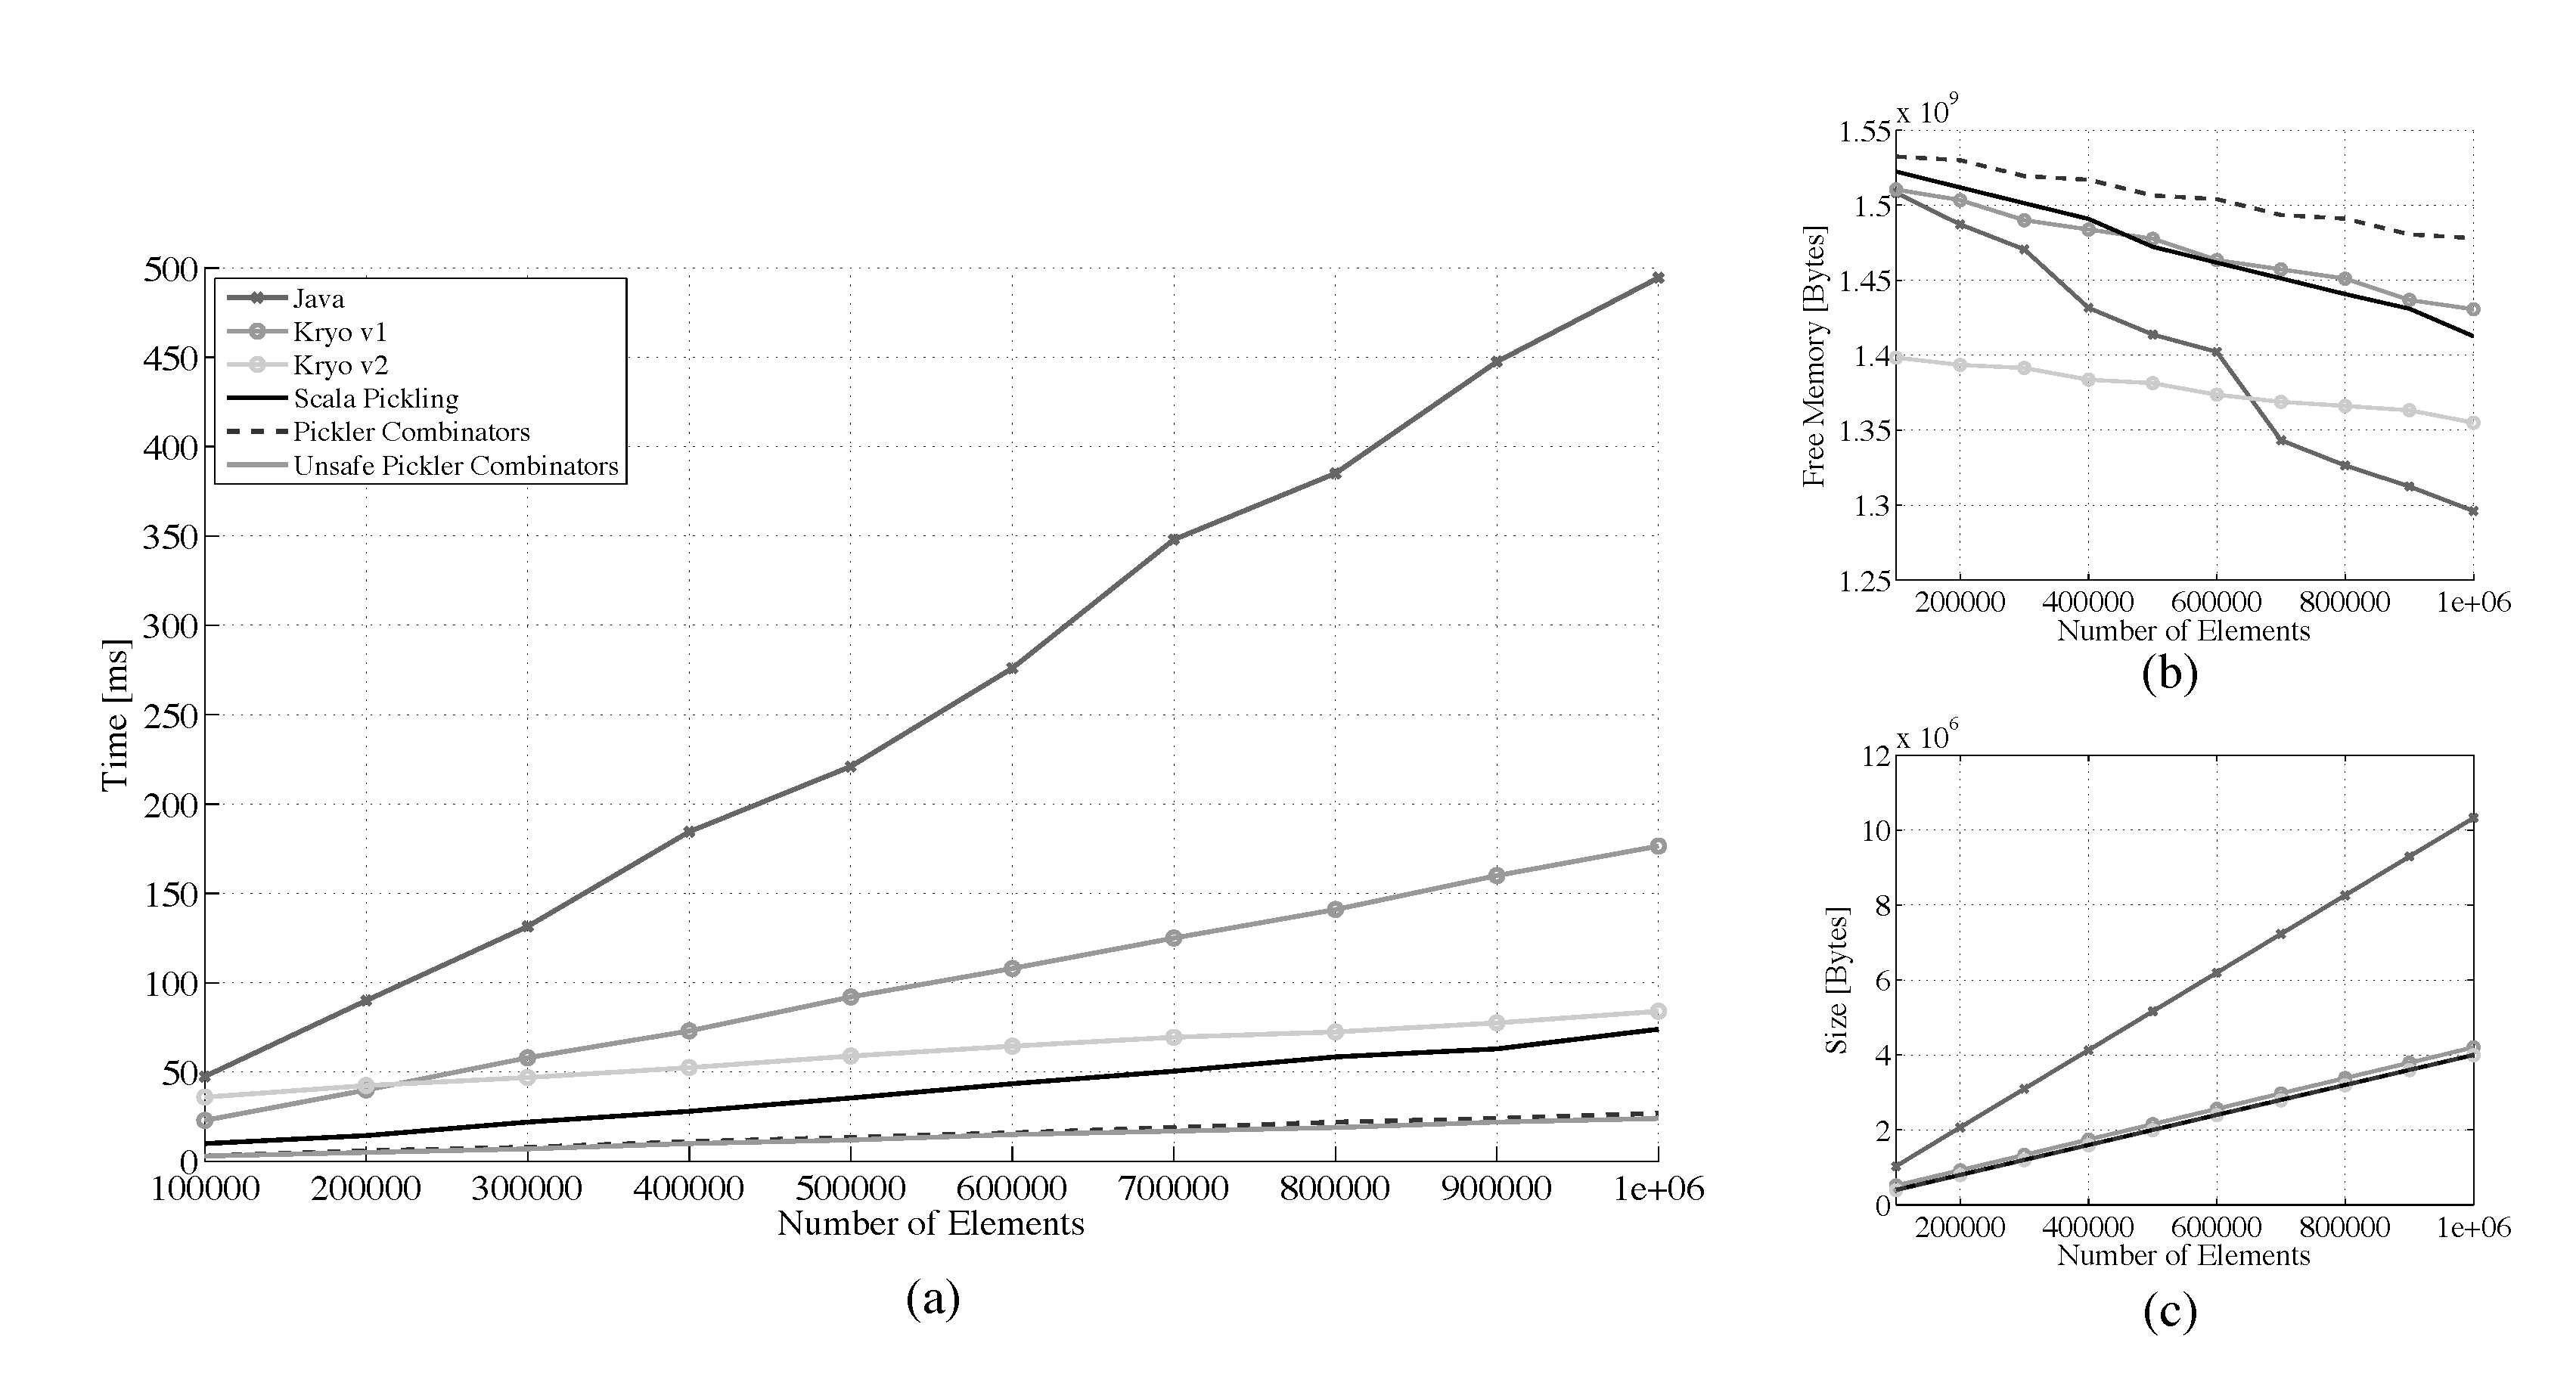
\includegraphics[width=\textwidth]{travInt-all.pdf}
 \caption{\footnotesize Results for pickling and unpickling an immutable
   \texttt{Vector[Int]} using different frameworks. Figure~\ref{fig:results-vector}(a) shows the roundtrip pickle/unpickle time as the size of the \texttt{Vector} varies. Figure~\ref{fig:results-vector}(b) shows the amount of free memory available during pickling/unpickling as the size of the \texttt{Vector} varies. Figure~\ref{fig:results-vector}(c) shows the pickled size of \texttt{Vector}.}
 \label{fig:results-vector}
\end{figure*}

In experiments, we've shown a naive, unoptimized version of Scala/Pickling
outperforming even the fastest serialization frameworks used in industry in time, space, and memory, as shown in Figure~\ref{fig:results-vector}.

Our results were accepted at OOPSLA 2013~\cite{Pickling}, a top-tier venue for programming languages research. I was the lead author on the project, conceived of the idea and lead the development with two colleagues to realize the implementation of Scala/Pickling.

\vspace{-0.2in}
\subsection*{\textbf{Spores}}
\vspace{-0.1in}

Spores are  functions that that

\vspace{-0.2in}
\subsection*{\textbf{Impact}}
\vspace{-0.1in}

I've additionally gone on to speak about Scala/Pickling I've, a recently minted professor of Computer Science and creator of \href{https://spark.incubator.apache.org/}{Apache Spark}~\cite{Spark} a framework for big data processing that's faster and rivals Hadoop/MapReduce

and released our framework fo, which exp

% Given the large number of , and Scala's penchant for

% With the growing trend towards cloud computing and mobile applications,
% distributed programming has entered the mainstream. Whether we consider a
% cluster of commodity machines churning through a massive data-parallel job, or
% a smartphone interacting with a social network, all are ``distributed'' jobs.
% % ,
% and all share the need to communicate in various ways, in many formats, even
% within the same application.

loded in popularity and has 300 stars and a dozen or so contributors to date.


Will enable functional programming languages like Scala to safely and reliably
\textit{distribute} their functional features.

Given that my research is also intended

This makes it possible to more reliably


\section*{\textbf{Essay 3:} Exhibiting Leadership: Bringing Twitter and Typesafe Engineers Together}

Pushed the \verb|Try| type into the now widely-used Scala Futures library.
Worked together with engineers at Twitter, Typesafe, and EPFL to standardize
and agree on a foundation for concurrency that is now included and ships with
the Scala Standard Library.

\section*{\textbf{Essay 4:} In Pursuit of Anita's Goal of 50/50 by 2020}

\textbf{Computing should be seen as creative and captivating.}
After all, Computer Science is at heart the of beguiling and mind-bending new
fields like {Brain-Computer} Interfacing -- where, with non-invasive imaging
modalities such as EEG, users are able to play video games, type on a virtual
keyboard, pilot robots, and more, using thoughts alone.

Why is it then that popular culture depicts those who work in the field of
computing so undesirably? Harrowing images abound; men sporting apparel
fashionable in IBM's hallways during the eighties, wearing glasses with
aviator-sized lenses and thick clear plastic frames, hunched before a large
and yellowed CRT monitor. Or perhaps worse, the more recent and unfortunate
stereotype of male developers as a {single-bodied} {beer-guzzling},
{pizza-swallowing} mass, famously gender/sexuality/etc. insensitive at
hackathons and conferences -- an image that is sometimes a reality in
some of Silicon Valley's communities, and which begot the {now-standard} ``code
of conduct'' sported by most all developer events.

With images like these permeating popular culture, it's no wonder that teenage
girls might be deterred from selecting Computer Science as a major in college.
It's natural to imagine that they might feel like they wouldn't fit in,
despite potentially even having an innate inclination for mathematics,
computers, or technology. In fact,
\href{https://www.girlscouts.org/research/pdf/generation\_stem\_full\_report.pdf}{Girl Scouts of America found}
\cite{Girlscouts} that a whopping 74\% teenage girls are indeed interested in {\em
Science, Technology, Engineering, and Mathematics} (STEM) fields, but about
half feel that STEM isn't a typical career path for girls. 57\% of teenage
girls surveyed say that if they went into a STEM career, they feel they'd have
to work harder than a man to be taken seriously. Worse, 13\% of those
interested in pursuing a STEM career say it's their first choice.

These numbers ripple surprisingly well through to reality. Here at EPFL, for
instance, our bachelors and masters programs are typically comprised of only
\href{http://www.swissict.ch/fileadmin/award/Impressionen/Symposium/WillyZwaenepoel\_ICT-Akademie.pdf}{$7\%$}~\cite{Willy}
women. Our PhD program fares slightly better; due to an initiative to
encourage applications from women, we can proudly tout a student body
comprised of $\approx15\%$ women. These numbers are simply not enough.

While EPFL can tout the existence of a handful of initiatives aimed at
encouraging women to apply for its Computer Science programs, or at retaining
women in PhD programs, their ultimate effects are less than stellar. For
instance, ``Robots for Girls'', a workshop aimed at teaching girls how to
program small robots, is EPFL's only program designed to foster interest
amongst girls in technology,
% (and to ultimately encourage them to apply to EPFL)
and it reaches at most 40 girls aged 11-13 years per year.
For PhD students, ``StartingDoc'' is a university-wide support group designed
to help women navigate through the labyrinth that is their first few years of
grad school; only one to two women from Computer Science participate each year.
As a participant in at least one of these initiatives, I'm not convinced that
they have enough of an observable effect to make a meaningful difference.

% Perhaps we should instead ask ourselves why we don't do more to change how
% young people perceive our field.

\textbf{To engage more young women, we need to change the image of our field,
and the way we encourage young women to join it.}

Given the opportunity to make a meaningful impact in this space, as Head
of EPFL's Computer Science Department, I'd focus on \textit{recruitment} and
\textit{retainment}.

\vspace{-0.15in}
\subsection*{\textbf{Recruitment}}
\vspace{-0.1in}
We need to demonstrate that computing is a captivating and creative field, and
we need to do it with strong and inspirational women role models.

\textit{\textsf{Local ``Maker's Faires''}}\newline
I'd team up with other departments at EPFL such as Electrical Engineering,
Mechanical Engineering, Manufacturing Engineering, and Physics to found a
large, {bi-yearly} event similar in spirit to what's known in the US as
\href{http://news.cnet.com/8301-13772_3-9935358-52.html}{\textit{Maker's
Faires}}; vivacious multi-day events desiged to ``celebrate arts, crafts,
engineering, science projects and the Do-It-Yourself (DIY) mindset''
\cite{MakerFaire}. A primary goal would be to encourage participation of
young women from local high schools and communities; to achieve this, we'd
engage with local schools, and would support all female attendees.

The goal of the events would be to inspire and amaze attendees, and to
introduce countless different facets of engineering and computing under a
creative guise. We'd achieve it through dozens of workshops aimed at
introducing a new tool, like 3D printing or Arduino or Raspberry Pi
programming, and imaginative use-cases for them. We'd invite dozens of
energetic demonstrations from within and outside the EPFL community, showing
off home-made electronic or computer musical instruments, or remote-control
small-scale battleships that the attendees can interact and battle with, to
name a few potential examples. To top it off, we'd have a full program of
talks featuring prominent and infectiously inspirational ``makers''; folks
(predominantly women) who have taken their creative technical edge to some
length of greatness.

\textit{\textsf{Open Houses}}\newline
For students electing to join EPFL, we'd turn our annual Open House events
into {small-scale} Maker's Faires, inviting EPFL labs and prominent makers
from afar to give energetic workshops, talks, and demonstrations. For these
events, we'd put together a special Computer Science showcase, showing
off cool, creative DIY projects with computing at their core, as well as
captivating Computer Science research projects, like some of the mind-blowing
research being done in robotics at EPFL.

\textit{\textsf{Role Models}}\newline
Most importantly, I'd ensure that at least half of the speakers joining both
types of events were \textit{creative}, \textit{energetic}, and
\textit{passionate} woman ``makers''. Having struggled intensely myself at the
onset of my career in Computer Science trying to find my place, I understand
how important it is to have real role models that can connect with young women
in person.
% Without them, it can be impossible to gauge what's normal or to
% see what's possible in one's career.

It's actually precisely for this reason, that in my own life, I have answered
a calling as a \textit{technical} speaker at prestigious industrial events,
like Strange Loop 2013 and Scala Days 2013. It's immensely important to me to
demonstrate to women at large that we can be strong, beautiful, and passionate
\textit{technical}  ``makers'' too -- that it's not just cool, it's \textit{normal}!


% Outfits like MIT's Media Lab regularly set out to change the way we
% interact with technology, captivating the world every step of the way; from
% \href{http://tangible.media.mit.edu/project/inform/}{a new haptic interface
% which renders 3D content physically, so users can interact with digital
% information in a tangible way} \cite{inFORM} to
% \href{http://www.media.mit.edu/research/groups/1458/cityscope}{an urban design
% system which combines simulation technology, 3D projection mapping, and
% physical models} \cite{CityScope}.

% from Make magazine and
% the worldwide movement of events like ``Makers Faires'' Women like 23 year old
% Zina Nichole Lahr have inspired hundreds of thousands, using technology to
% drive her own animations.

\vspace{-0.15in}
\subsection*{\textbf{Retainment}}
\vspace{-0.1in}

Appealing to and drawing in women isn't our only challenge as educators in
Computer Science -- retaining them has also proven to be an enormous obstacle.
At Stanford University, during the 2012-2013 school year for example, 40\% of
the introductory CS course was female, which subsequently dropped to 30\% in
part 2 of the same course, then down again to 20\% in part 3. Computer Science
overall at Stanford is merely 12\% female~\cite{ShePlusPlus}.

The field is fraught with challenges, even at the undergraduate level, from
\href{http://www.pgbovine.net/tech-privilege.htm}{micro-inequities}~\cite{MicroInequities} to
\href{http://www.networkworld.com/news/2012/061312-gmail-women-260169.html}{Impostor Syndrome}~\cite{ImpostorSyndrome}
to name only some intrinsic trials and tribulations that women in Computer
Science face.

To retain young women in Computer Science at EPFL, I'd initiate an extensive
support net for our female students, which would involve female faculty in the
department. Having myself struggled with direction and adversity as an
undergraduate, I can attest to the power of a mentor's advice and attention --
for many, it takes only a bit of advice or encouragement to catapult a
student from distress and feelings of ineptitude to self-confidence and
triumph.

Female faculty would meet at least once per semester; together, we would
venture through the list of all female students in the department to discuss
how well each student is doing, and what the department could do for those
young women who seem to be dwindling in motivation or perseverance.

\vspace{-0.15in}
\subsection*{\textbf{In Sum}}
\vspace{-0.1in}

I deeply and passionately believe that the way forward to realizing Dr. Anita
Borg's and so many others' goal of equal participation is to work together to
change our profession's image. We must strive to induce excitement, and to
show all of the exhilarating and creative things that can be undertaken in
computing. And to get there, we need a brave batch of creative and motivated
women to lead the way, to show the world that this \textit{is} the norm.

Striving towards these goals is at the foundation of who I am. These goals
drive my decisions to give talks, talk to and interact with people in my
field, to write and tweet. They will continue to be a motivating force for me
in my career for as long as imbalance abounds.

% \bibliographystyle{siam}
% \bibliographystyle{plain}
% \bibliography{bib}

\printbibliography
% \printbibheading
% \printbibliography[type=book,heading=subbibliography,title={Books}]
% \printbibliography[type=article,heading=subbibliography,title={Journal Articles}]
% \printbibliography[type=inproceedings,heading=subbibliography,title={Conference and Workshop Papers}]
% \printbibliography[nottype=book,nottype=article,nottype=inproceedings,heading=subbibliography,title={Other Sources}]

% \begin{received}
% Prepared January 2011
% \end{received}

\end{document}


